

\chapter[追踪算法设计]{追踪算法设计}[Harbin Institute of Technology Postgraduate Dissertation Writing Specifications]

算法设计核心为高效、准确。尽管基于深度学习的方法\citep{zhang2021fairmot,meinhardt2022trackformer,li2019evolution,zhou2020tracking,bewley2016simple}可以得到非常高的准确率,然后其对于计算资源的开销也是不可忽视的,
因此在算法设计过程中并没有考虑引入深度学习的思路。\par
算法设计思路为:为每块装甲板单独建立运动模型,每块有运动模型的装甲板利用运动模型对当前时刻进行位置预测,然后与观测到的装甲板进行一一配对,若距离小于阈值且观测装甲板的数字与携带运动模型对应装甲板的数字一致,
则认为两者同属一块装甲板,利用当前装甲板信息更新运动模型,从而实现追踪效果。
为了实现追踪效果的鲁棒性,允许装甲板的运动模型在短时间不更新,从而起到在受遮挡的情况下依然保留运动模型,待装甲板离开遮挡后不必重新计算运动模型;但是较长时间不更新则认为目标已经不在视野范围内。
\par

另外追踪层级有两层,第一级为追踪同一块装甲板,若追踪同一块装甲板失败,则退而求其次,追踪同一辆车。追踪逻辑如图\ref{追踪算法逻辑图}所示:

\begin{figure}[H]
    \centering
    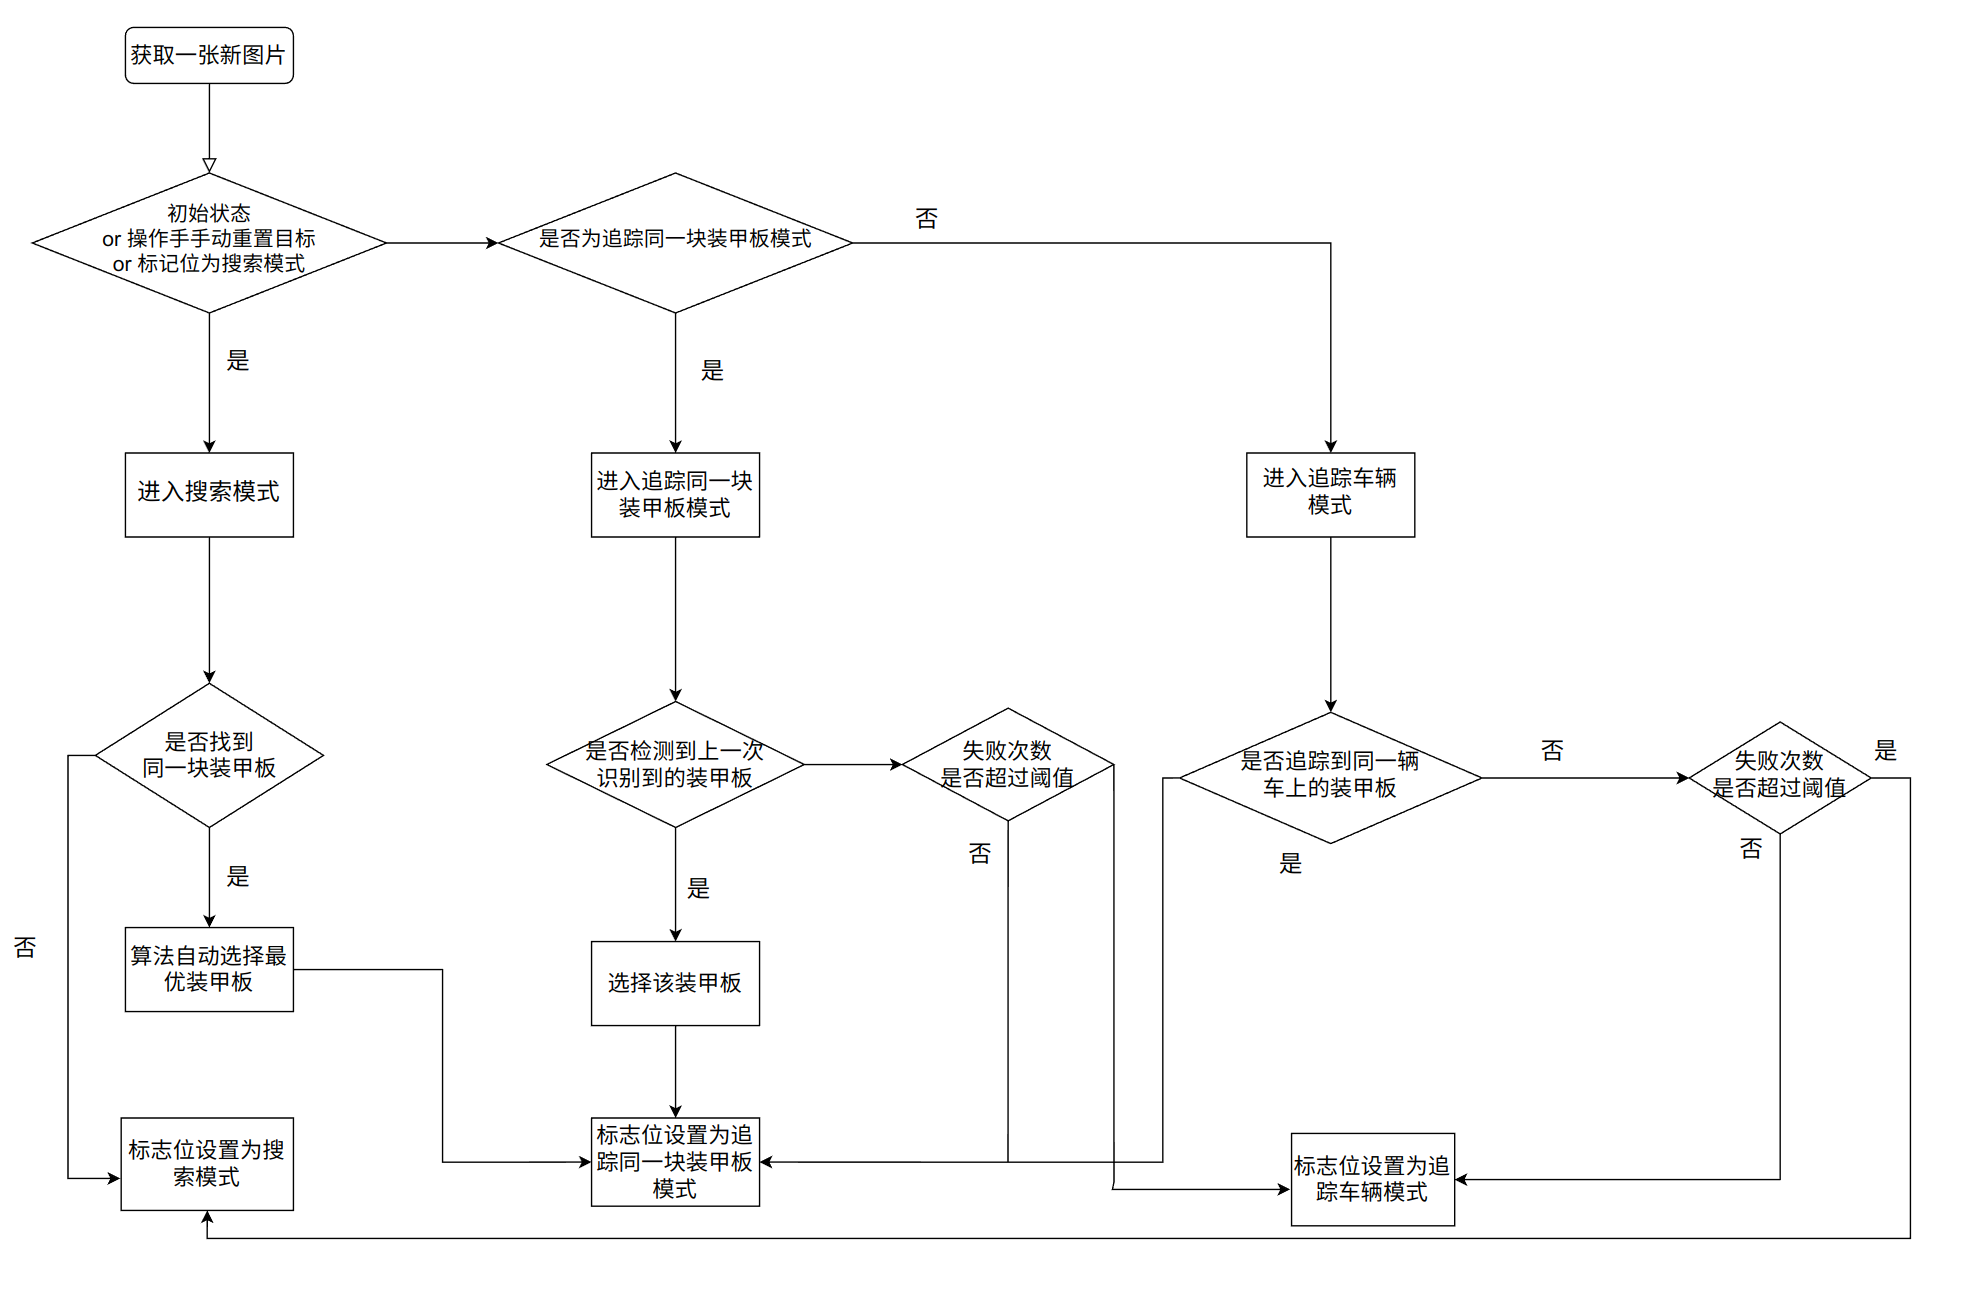
\includegraphics[width=.8\textwidth]{track_chart.png} 
    \caption{追踪算法逻辑图} 
    \label{追踪算法逻辑图} 
\end{figure} 


